\documentclass[11pt]{article}

\usepackage[lf]{Baskervaldx} % lining figures
\usepackage[bigdelims,vvarbb]{newtxmath} % math italic letters from Nimbus Roman
\usepackage[cal=boondoxo]{mathalfa} % mathcal from STIX, unslanted a bit
\renewcommand*\oldstylenums[1]{\textosf{#1}}

\usepackage[framed]{matlab-prettifier}

\usepackage{amsmath}
\usepackage{amssymb}
\usepackage{parskip}
\usepackage{bm}
\usepackage[a4paper,hmargin=1in,vmargin=1in]{geometry}

\usepackage{graphicx}
\usepackage{color}

\usepackage[hyphens]{url}
\usepackage[colorlinks,linkcolor=red,anchorcolor=black,citecolor=blue]{hyperref}

\newcommand{\alp}{\ensuremath{\alpha}}

\begin{document}

\section*{Problem 4}

\subsection*{4.1}

The problem is convex, as it maximizes of a concave function (the CRRA utility function) over a convex set ($[\underline{\alp},\bar{\alp}] \in \mathbb{R}$). Thus, a Kuhn-Tucker method can be applied to solve the problem.

\subsection*{4.2}

Without the constraint, the first-order condition implies $$\mathbb{E} [w_0^\phi (1+ r^f + \alp(r-r^f))^{\phi-1} (r-r^f)] = 0.$$ But since $w_0$ is a constant, it can be taken out of the expectation operator, and so the optimal share $\alp$ is independent of the initial wealth $w_0$, which is a property of the CRRA utility.

Now the condition can be rewritten as $$ p [1+ r^f + \alp(r_{low}-r^f)]^{\phi-1} (r_{low}-r^f) + (1-p) [1+ r^f + \alp(r_{high}-r^f)]^{\phi-1} (r_{high}-r^f) = 0. $$ Use Matlab function \emph{fzero}, the optimal value is reached at $a^* = 2.7331 $, and the plot of $\alp$ against the value of the objective (wlog $w_0 = 1$) looks like:
\begin{figure}[h!]
\centering
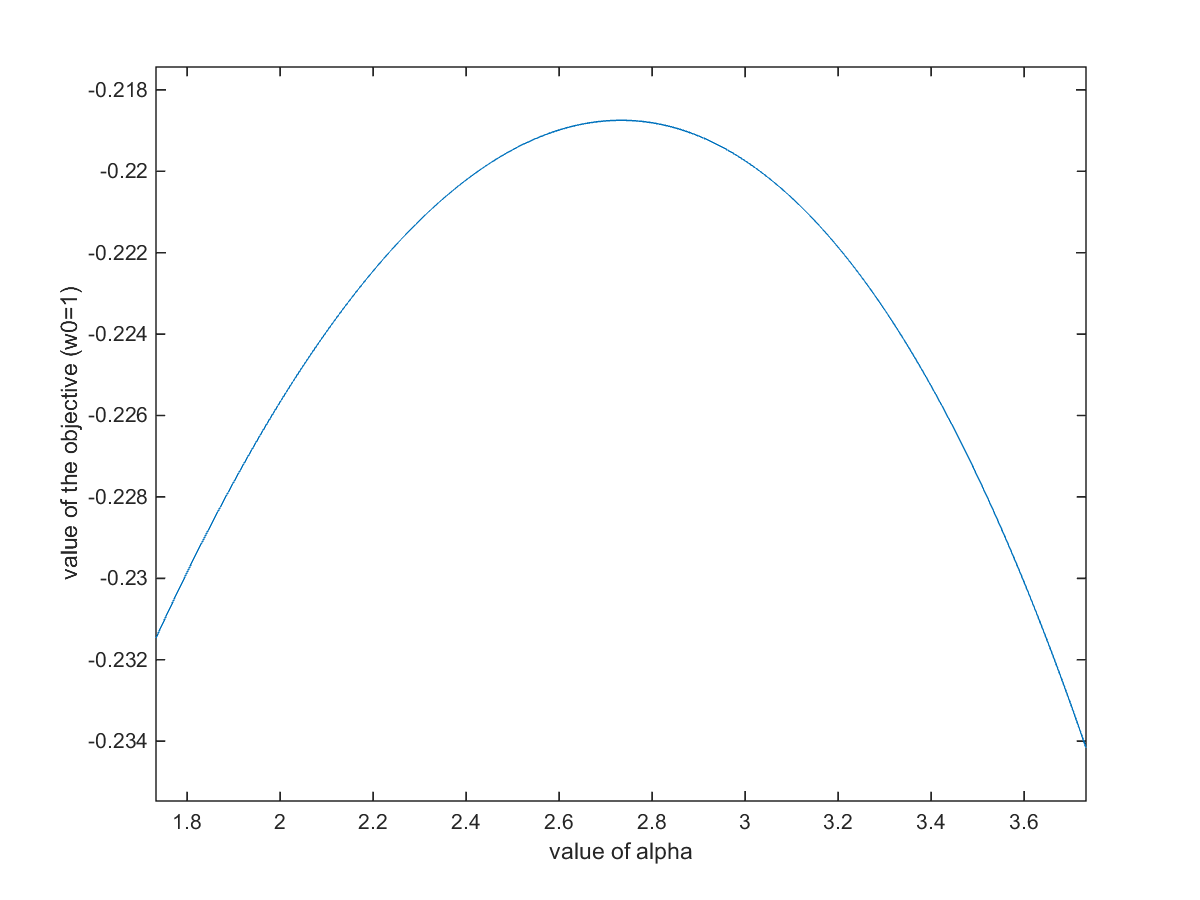
\includegraphics[width=0.6\textwidth]{plot42}
\end{figure}

\subsection*{4.3}

The lower bound $\underline{a} = 0$ implies that investor cannot be on the short position, and the upper bound $\bar{a} = 1$ means that the investor cannot borrow money to buy the risky asset.

In Matlab, \emph{fmincon} finds the minimum of constrained nonlinear multivariable function, while \emph{fminbnd} finds the minimum of single-variable function on fixed interval. Clearly, \emph{fmincon} is far more advanced than what is required for this problem. Starting from the initial value $\alp = 0.5$, the two methods gave the same result $\alp^{**} = 1$.

The intuition is straightforward: since the unconstrained optimum $a^*>1$, and since the function is increasing in $[0,1]$, the best strategy under the constraint is to hit the right bound, i.e. invest all in the risky asset.

\appendix

\section*{Matlab codes}

\subsection*{Problem 4}

\begin{lstlisting}[style=Matlab-editor]
syms a;
rf = 0.02; rlr = -0.08-rf; rhr = 0.12-rf;
p = 0.1; phi = -3;

f = -(p*(1 + rf + a*rlr)^phi + (1 - p)*(1 + rf + a*rhr)^phi)/phi;
df = diff(f,a);
mf = matlabFunction(f);
mdf = matlabFunction(df);
astar1 = fzero(mdf,1);
display(['The unconstrained solution is ', num2str(astar1)]);

figure;
set(gcf,'color','w');
ezplot(-f,[astar1-1,astar1+1]);
xlabel('value of alpha');
ylabel('value of the objective (w0=1)');
title('');
print('plot42','-dpng')

astar2 = fminbnd(mf,0,1);
astar3 = fmincon(mf,0.5,[],[],[],[],0,1);
display(['The function fminbnd and fmincon give the constrained solution ', num2str(astar2), ' and ', num2str(astar3)]);
\end{lstlisting}



\end{document}

